\documentclass[]{book}
\usepackage{lmodern}
\usepackage{amssymb,amsmath}
\usepackage{ifxetex,ifluatex}
\usepackage{fixltx2e} % provides \textsubscript
\ifnum 0\ifxetex 1\fi\ifluatex 1\fi=0 % if pdftex
  \usepackage[T1]{fontenc}
  \usepackage[utf8]{inputenc}
\else % if luatex or xelatex
  \ifxetex
    \usepackage{mathspec}
  \else
    \usepackage{fontspec}
  \fi
  \defaultfontfeatures{Ligatures=TeX,Scale=MatchLowercase}
\fi
% use upquote if available, for straight quotes in verbatim environments
\IfFileExists{upquote.sty}{\usepackage{upquote}}{}
% use microtype if available
\IfFileExists{microtype.sty}{%
\usepackage{microtype}
\UseMicrotypeSet[protrusion]{basicmath} % disable protrusion for tt fonts
}{}
\usepackage[margin=1in]{geometry}
\usepackage{hyperref}
\hypersetup{unicode=true,
            pdftitle={Guide d'organisation d'un data sprint},
            pdfauthor={Samuel Goëta (Datactivist) pour le lab 110bis du ministère de l'Éducation nationale},
            pdfborder={0 0 0},
            breaklinks=true}
\urlstyle{same}  % don't use monospace font for urls
\usepackage{natbib}
\bibliographystyle{apalike}
\usepackage{longtable,booktabs}
\usepackage{graphicx,grffile}
\makeatletter
\def\maxwidth{\ifdim\Gin@nat@width>\linewidth\linewidth\else\Gin@nat@width\fi}
\def\maxheight{\ifdim\Gin@nat@height>\textheight\textheight\else\Gin@nat@height\fi}
\makeatother
% Scale images if necessary, so that they will not overflow the page
% margins by default, and it is still possible to overwrite the defaults
% using explicit options in \includegraphics[width, height, ...]{}
\setkeys{Gin}{width=\maxwidth,height=\maxheight,keepaspectratio}
\IfFileExists{parskip.sty}{%
\usepackage{parskip}
}{% else
\setlength{\parindent}{0pt}
\setlength{\parskip}{6pt plus 2pt minus 1pt}
}
\setlength{\emergencystretch}{3em}  % prevent overfull lines
\providecommand{\tightlist}{%
  \setlength{\itemsep}{0pt}\setlength{\parskip}{0pt}}
\setcounter{secnumdepth}{5}
% Redefines (sub)paragraphs to behave more like sections
\ifx\paragraph\undefined\else
\let\oldparagraph\paragraph
\renewcommand{\paragraph}[1]{\oldparagraph{#1}\mbox{}}
\fi
\ifx\subparagraph\undefined\else
\let\oldsubparagraph\subparagraph
\renewcommand{\subparagraph}[1]{\oldsubparagraph{#1}\mbox{}}
\fi

%%% Use protect on footnotes to avoid problems with footnotes in titles
\let\rmarkdownfootnote\footnote%
\def\footnote{\protect\rmarkdownfootnote}

%%% Change title format to be more compact
\usepackage{titling}

% Create subtitle command for use in maketitle
\providecommand{\subtitle}[1]{
  \posttitle{
    \begin{center}\large#1\end{center}
    }
}

\setlength{\droptitle}{-2em}

  \title{Guide d'organisation d'un data sprint}
    \pretitle{\vspace{\droptitle}\centering\huge}
  \posttitle{\par}
    \author{Samuel Goëta (Datactivist) pour le lab 110bis du ministère de
l'Éducation nationale}
    \preauthor{\centering\large\emph}
  \postauthor{\par}
      \predate{\centering\large\emph}
  \postdate{\par}
    \date{2019-04-18}

\usepackage{booktabs}

\begin{document}
\maketitle

{
\setcounter{tocdepth}{1}
\tableofcontents
}
\chapter{Introduction}\label{introduction}

A la suite du dataviz challenge organisé les 22 et 23 mars 2019, le
guide d'organisation d'un data sprint doit : * Permettre l'essaimage du
format au sein du Ministère de l'Education nationale et de la Jeunesse
et auprès de ses partenaires ainsi que dans les territoires * Rendre
l'évènement réplicable * Restituer l'expérience du dataviz challenge et
inciter d'autres acteurs à le reproduire.

Le guide est open source, il s'appuie sur le
\href{https://docs.google.com/document/d/1uDw4Maifjl_egJ95y-F0dkXEyu2MNfhc2GvNEmjhPq8/edit\#heading=h.9ofnjz67swln}{travail
réalisé par Datactivist pour le département de l'Ardèche} sous licence
\href{https://creativecommons.org/licenses/by-sa/4.0/deed.fr}{CC BY-SA
4.0} (Attribution - Partage dans les Mêmes Conditions 4.0
International). Le guide est publié avec la même licence qui permet la
libre réutilisation tout en garantissant que le contenu restera ouvert.

Pour favoriser la réplication de l'évènement, le guide comprend des
conseils méthodologiques ainsi que des documents type qui faciliteront
l'organisation de ce type d'évènements.

\section{Le contenu du guide}\label{le-contenu-du-guide}

\chapter{Le dataviz challenge : un évènement à répliquer}\label{dataviz}

Le dataviz challenge s'est inscrit dans le cadre de la mission relative
aux politiques éducatives territoriales confiée en octobre 2018 par le
ministre de l'Education nationale et de la Jeunesse, Jean-Michel
Blanquer, à Ariane Azéma, inspectrice générale de l'administration de
l'éducation nationale et de la recherche et à Pierre Mathiot, professeur
des universités.

Il part du constat que la concentration géographique des inégalités
sociales et ses effets sur l'échec scolaire est identifiée depuis de
nombreuses années en France : elle est un des fondements historiques des
politiques d'éducation prioritaire. Le ministère doit procéder à la
révision de la carte de la géographie prioritaire et veut, plus
globalement, mieux prendre en compte l'ensemble des enjeux territoriaux
qui contribuent à la réussite de tous les élèves.

Dans le cadre de cette mission, le
\href{https://www.education.gouv.fr/110bislab/cid130754/presentation-du-110-bis-lab-d-innovation-de-l-education-nationale.html}{110
bis}, lab d'innovation de l'Education nationale, a expérimenté du
vendredi 22 mars 9h au samedi 23 mars 19h un nouveau format
d'exploitation de données visant à co-construire des outils, une
méthodologie et des pratiques pour améliorer les politiques publiques
éducatives.

L'évènement s'adressait à un large public : développeur, enseignant,
data scientist, designer, chercheur, professionnel de l'éducation,
décideur public, étudiant, et quiconque souhaitant apporter sa
contribution sur le sujet des politiques éducatives territoriales et
s'immerger dans une équipe interdisciplinaire le temps des deux jours du
dataviz challenge.

\begin{figure}

{\centering 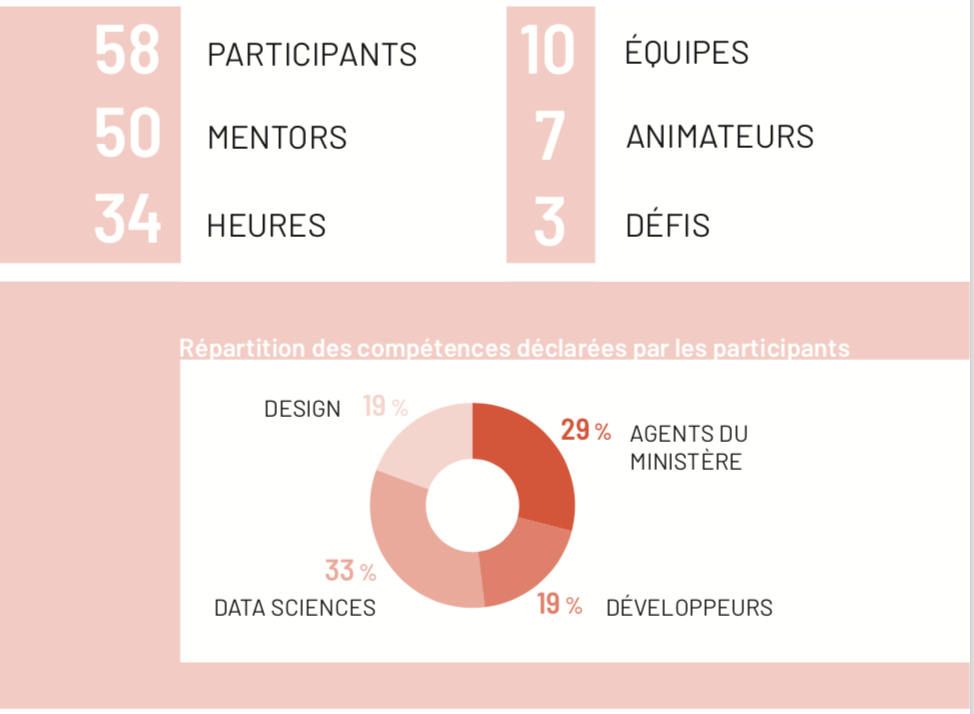
\includegraphics[width=0.5\linewidth]{./img/participants} 

}

\caption{Extrait du livret du dataviz challenge représentant la diversité des participants}\label{fig:unnamed-chunk-1}
\end{figure}

Les 3 défis du dataviz challenge ont été identifiés lors d'une journée
contributive le 3 octobre 2018 avec les acteurs de terrain.

Les défis 1 et 2 se sont appuyés sur des données qui ne sont pas
librement réutilisables en open data. Bien qu'anonymisées, ces données
concernaient des personnes physiques ou morales et les participants se
sont engagés à ne pas ni altérer les données, ni dénaturer leur sens et
à présenter les résultats de manière à ne pas permettre une éventuelle
identification.

\section{Défi 1 : «Les déplacements en
cascade»}\label{defi-1-les-deplacements-en-cascade}

\subsection{Cadrage du défi}\label{cadrage-du-defi}

L'émergence des campus des métiers et des qualifications, le
développement de l'apprentissage, la réforme du lycée, etc. sont autant
de politiques publiques éducatives qui peuvent se traduire par la
modification de l'offre de formation sur le territoire. Comment
représenter les conséquences potentielles de ces modifications sur les
déplacements des élèves et des professeurs ?

\textbf{Objectifs} : anticiper les impacts plausibles d'une modification
de l'offre de formation au niveau local, sur les déplacements des
professeurs et des élèves (nombre de personnes impactées, temps de
transport, etc.)

\textbf{3 questions pour démarrer le DataViz Challenge :}

\begin{itemize}
\item
  Comment mettre en regard le déplacement de l'offre de formation et
  l'offre de transports, dont une partie est gérée par les collectivités
  ?
\item
  Comment tenir compte et représenter les différentes stratégies qui
  peuvent être mises en oeuvre par les élèves ?
\item
  Quels sont les effets du déplacement d'une option ou d'une spécialité
  sur la mixité sociale ?
\end{itemize}

3 projets ont été développés dans le cadre de ce défi.

\subsection{\texorpdfstring{🏆 Projet ``Mixité
Sociale''}{🏆 Projet Mixité Sociale}}\label{projet-mixite-sociale}

\begin{quote}
\emph{Ce projet a été retenu par le jury pour le défi 1.} Lien vers le
code et la documentation : \url{https://github.com/kir0ul/DataTerr}
\end{quote}

\textbf{Contexte}

Au sein d'un périmètre restreint, des établissements peuvent être
caractérisés par des niveaux de mixité sociale, entendue comme la
représentation équilibrée de toutes les différentes professions et
catégories socioprofessionnelles (PCS), très inégaux.

A Bordeaux, trois collèges publics limitrophes ont des indices de mixité
respectifs de 30,4, 46,2 et 9,7 \%, tandis que la moyenne académique est
de 34,9\%.

Comment améliorer cet indice, notamment pour les établissements où il
demeure faible ? Comment identifier les variables sur lesquelles jouer
et leur impact plausible sur l'indice de mixité d'établissements proches
?

\textbf{Produit final} S'appuyant sur QGIS pour explorer les données,
l'équipe s'est focalisée sur la ville de Bordeaux car nous disposions
des données de carte scolaire. Chaque établissement est représenté par
ses indicateurs PCS, le nombre d'élève de secteur non présent dans
l'établissement, l'indicateur PCS\_D (catégories sociaux
professionnelles défavorisées) prédit par le modèle, et enfin
l'indicateur PCS\_D après déplacement d'options.

L'équipe avait aussi pour projet de développer également une aide à la
modification des cartes scolaires, non réalisée faute de temps.

\begin{figure}

{\centering 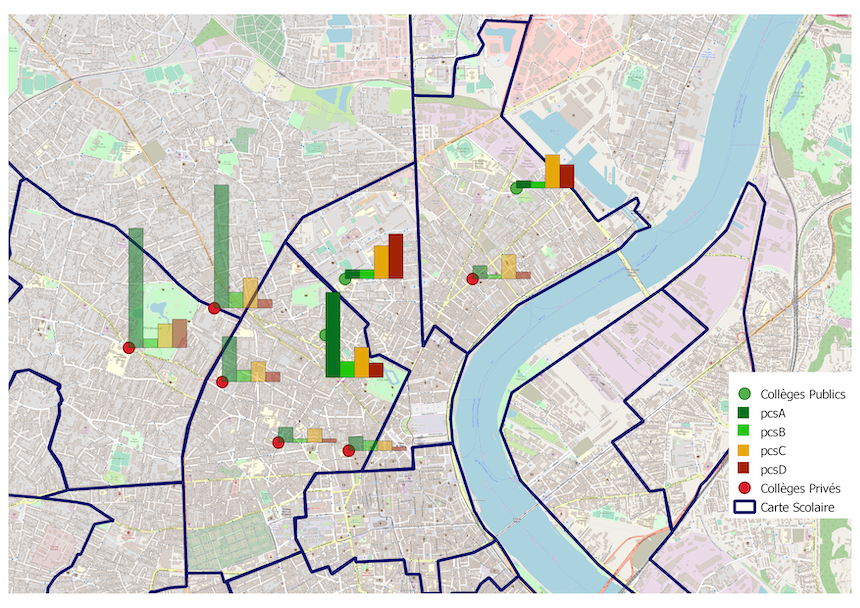
\includegraphics[width=0.6\linewidth]{./img/Diagramme_Publics_Prives} 

}

\caption{Exemple de carte prédisantle  niveau de mixité sociale}\label{fig:unnamed-chunk-2}
\end{figure}

\textbf{Méthode} Le modèle choisi est un
\href{https://fr.wikipedia.org/wiki/For\%C3\%AAt_d\%27arbres_d\%C3\%A9cisionnels}{régresseur
à base de forêts aléatoires}. La variable à prédire est le taux d'élèves
en PCS très défavorisé et les variables d'entrée sont le nombre
d'élèves, secteur/privé, le nombre d'options disponibles, et les options
d'intérêt.

\begin{figure}

{\centering 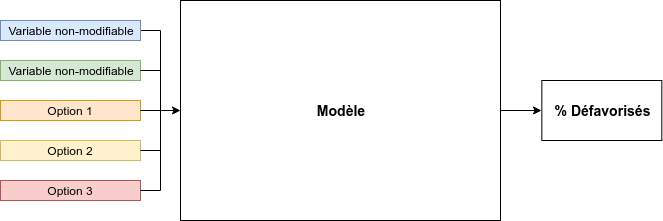
\includegraphics[width=0.6\linewidth]{./img/model-diag} 

}

\caption{Représentation synthétique du modèle}\label{fig:unnamed-chunk-3}
\end{figure}

Malgré la simplicité de cette sélection de variables, le modèle a une
\href{https://fr.wikipedia.org/wiki/Erreur_quadratique_moyenne}{erreur
RMSE}, mesure caractérisant la « précision » d'un estimateur, de 2\% ce
qui est très faible.

\begin{figure}

{\centering 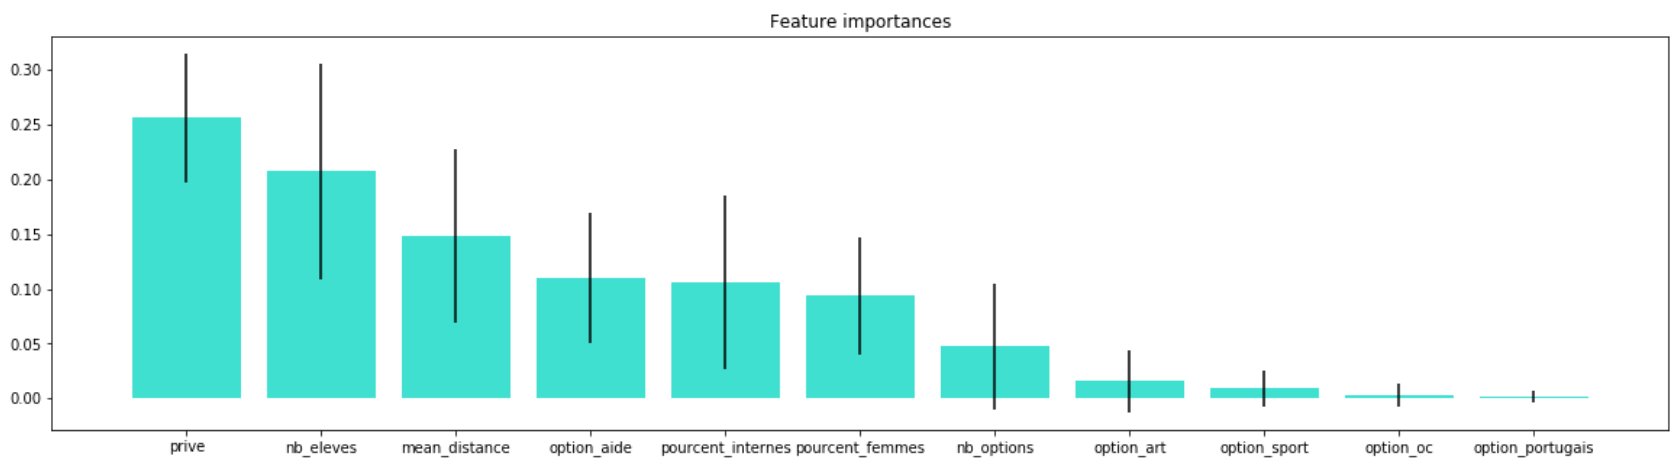
\includegraphics[width=1\linewidth]{./img/model-vars} 

}

\caption{Représentation sous forme de boite à moustache de la hiérarchisation automatique des variables utilisées par le modèle}\label{fig:unnamed-chunk-4}
\end{figure}

\subsection{\texorpdfstring{Projet
``Locaviz''}{Projet Locaviz}}\label{projet-locaviz}

\begin{quote}
\href{https://drive.google.com/file/d/1gpl02y7FG4hOCEh2t55YRlaRyTP010Pj/view?usp=sharing}{Lien
vers le code et la documentation du projet}
\end{quote}

\textbf{Contexte :} La fermeture ou l'ouverture d'un établissement
scolaire peut avoir de sérieux impacts sur les capacités d'accueil des
établissements similaires voisins, trajets quotidiens des élèves, et
donc sur des enjeux plus vastes tels que l'environnement.

Comment prévoir les impacts de la fermeture ou de l'ouverture d'un
établissement sur ces trois paramètres ?

\textbf{Produit final}: Une carte décrivant les impacts de la fermeture
d'un établissement sélectionné. En fonction du nombre de classes de
l'établissement, le prototype anticipe la réaffectation des élèves dans
les établissements environnants, ses impacts sur les trajets. Les
caractéristiques sociales de chaque établissement sont visualisées dans
une rosace qui se déplie par niveau.

\begin{figure}

{\centering 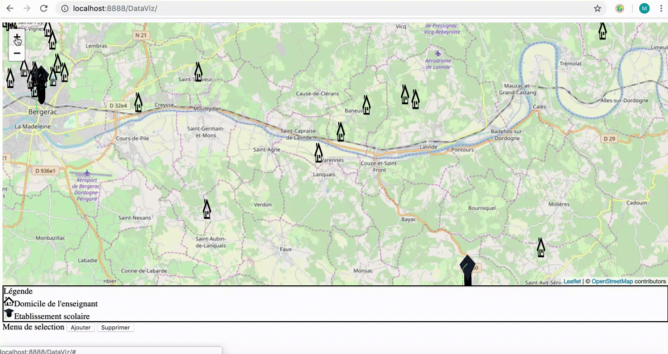
\includegraphics[width=0.6\linewidth]{./img/locaviz} 

}

\caption{Représentation cartographique de la suppression de la classe et des déplacements engendrés}\label{fig:unnamed-chunk-5}
\end{figure}

Le projet prévoit la réaffectation des élèves dans les établissements en
prenant en compte sa capacité actuelle et sa capacité après
réaffectation. Le temps de trajet n'a pu être calculé mais la distance
est représentée avec une estimation de l'impact carbone de ces
déplacements.

\subsection{Projet I.P.E.D. (Indice de Performance des
Déplacements)}\label{projet-i.p.e.d.-indice-de-performance-des-deplacements}

\begin{quote}
\href{http://datavizchallenge.fr/t/defi-numero-1-indice-annuel-d-evaluation-de-l-impact-mobilite-des-enseignants/131}{Lien
vers le code et la documentation}
\end{quote}

\textbf{Contexte} : Les enseignants qui exercent au sein de plusieurs
établissements, ou enseignants en compléments de services, doivent
souvent assumer de nombreux déplacements qui peuvent sensiblement peser
sur leur vie personnelle et professionnelle. A terme, cela peut avoir
des impacts notoires sur d'autres paramètres tels que l'environnement ou
les chances de réussite des élèves.

Comment analyser ces déplacements pour apporter des solutions efficaces
permettant de les limiter et d'en réduire les impacts?

\begin{figure}

{\centering 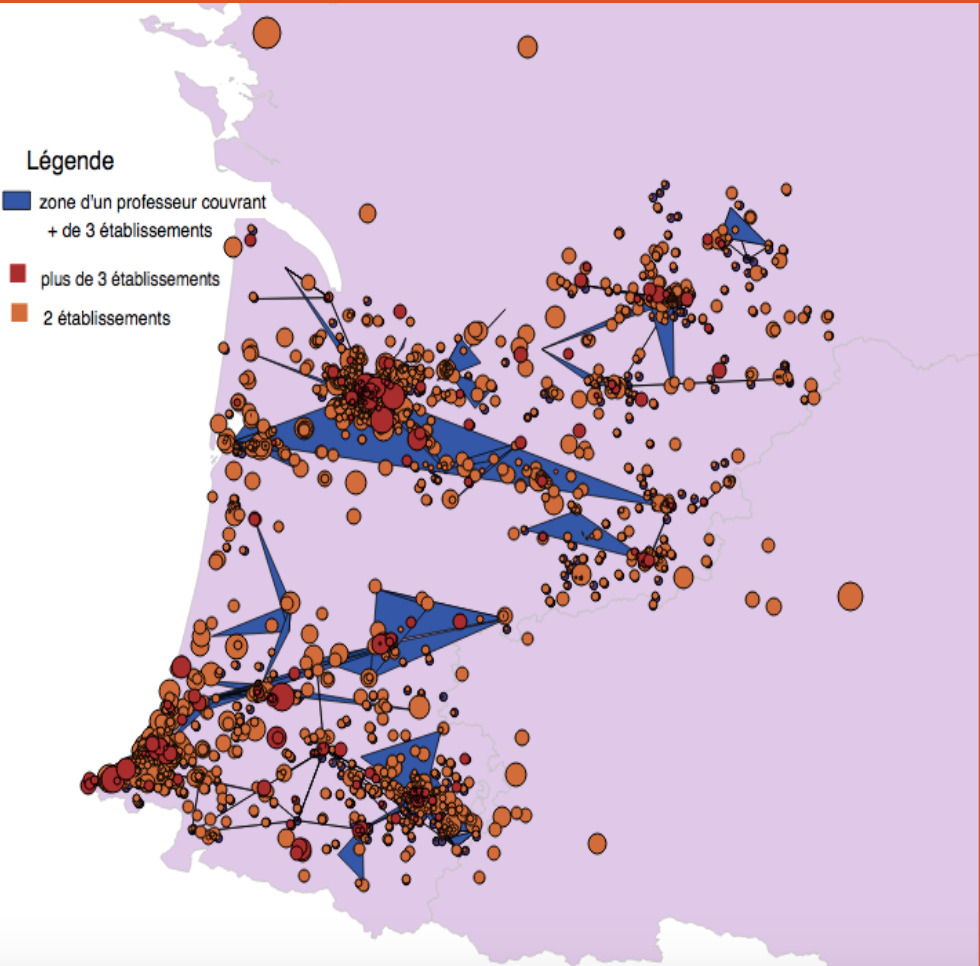
\includegraphics[width=0.6\linewidth]{./img/iped} 

}

\caption{Carte représentant les déplacements effectués par les enseignements en complément de service.}\label{fig:unnamed-chunk-6}
\end{figure}

\textbf{Produit Final} : Maquette de plateforme permettant de visualiser
l'évolution d'un Indice de Performance des Déplacements (IPED) en
fonction de l'évolution de paramètres qui déterminent l'offre éducative.

\begin{figure}

{\centering 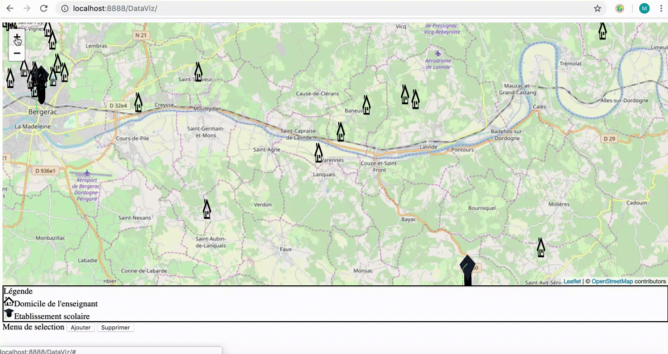
\includegraphics[width=0.6\linewidth]{./img/iped2} 

}

\caption{Maquette de la plateforme IPED.}\label{fig:unnamed-chunk-7}
\end{figure}

\textbf{Méthode} : Le projet a abouti à la création d'un indicateur IPED
:indice annuel, de base 100, d'évaluation de l'impact mobilité des
enseignants. Il se compose de l'addition globale des trajets à vol
d'oiseau de chacun.e des enseignant.e.s.

Selon le Lieu de résidence de l'enseignant, les matières et options
enseignées et la typologie de l'établissement, un algorithme recommande
un scénario d'optimisation des trajets.

\section{Défi N°2 : La carte d'identité des établissements en temps
réel}\label{defi-n2-la-carte-didentite-des-etablissements-en-temps-reel}

\subsection{Cadrage du défi}\label{cadrage-du-defi-1}

Les recteurs comme d'autres acteurs de l'Education nationale ont souvent
besoin de pouvoir prendre connaissance, en un coup d'oeil, de la
situation globale d'un établissement : l'état des ressources humaines et
financières, la situation sociale, les résultats des élèves, etc.
Comment remplacer une pile de dossiers papiers hétérogènes qui demandent
un effort considérable de constitution et de consultation, par une
vision synthétique, actualisée et à 360°, des informations relatives à
un établissement ?

\textbf{Objectifs} : avoir une vision consolidée et à jour d'un
établissement, diminuer le temps de préparation au profit du temps
consacré à l'échange, et ainsi faciliter le dialogue.

\textbf{3 questions pour démarrer le DataViz Challenge :}

\begin{itemize}
\tightlist
\item
  Comment synthétiser les informations nécessaires à la prise de
  connaissance de l'état d'un établissement ?
\item
  Comment permettre aux utilisateurs en mobilité (ex : recteurs) d'en
  disposer lors de leurs déplacements ?
\item
  Comment rendre cet outil utile pour des utilisateurs non experts de la
  donnée ?
\end{itemize}

\subsection{🏆Projet Eduscope}\label{projet-eduscope}

\begin{quote}
\emph{Ce projet a été retenu par le jury pour le défi 2.} Lien vers
l'outil : \url{https://avouacr.shinyapps.io/eduscope_shinyapp} Lien vers
le code et la documentation : \url{https://github.com/avouacr/EduScope}
\end{quote}

\textbf{Contexte} : Les recteurs, agents du ministère ou chefs
d'établissement ont souvent besoin d'obtenir rapidement des informations
sur les caractéristiques générales et les spécificités d'un
établissement cible. Aujourd'hui ces informations se trouvent dispersées
et stockées dans différentes bases de données (ex: GAIA, Mosart,
EPI\ldots{}), ce qui limite leur accessibilité, leur lisibilité et peut
donc complexifier la prise de décision.

Quel outil pourrait donc répondre aux besoins des différents
utilisateurs que sont: la visualisation rapide d'indicateurs, la
mobiquité et l'aide à la prise de décisions ?

\textbf{Produit final} : Plateforme interactive qui permet de
centraliser et de visualiser divers indicateurs de performance scolaire.
La priorisation des indicateurs d'intérêt s'adapte en fonction du profil
utilisateur (recteur, chef d'établissement, service support\ldots{}) et
de l'échelle de prise de décision souhaitée (nationale, académique,
département, bassin, établissement), tout en demeurant flexible.

\begin{figure}

{\centering 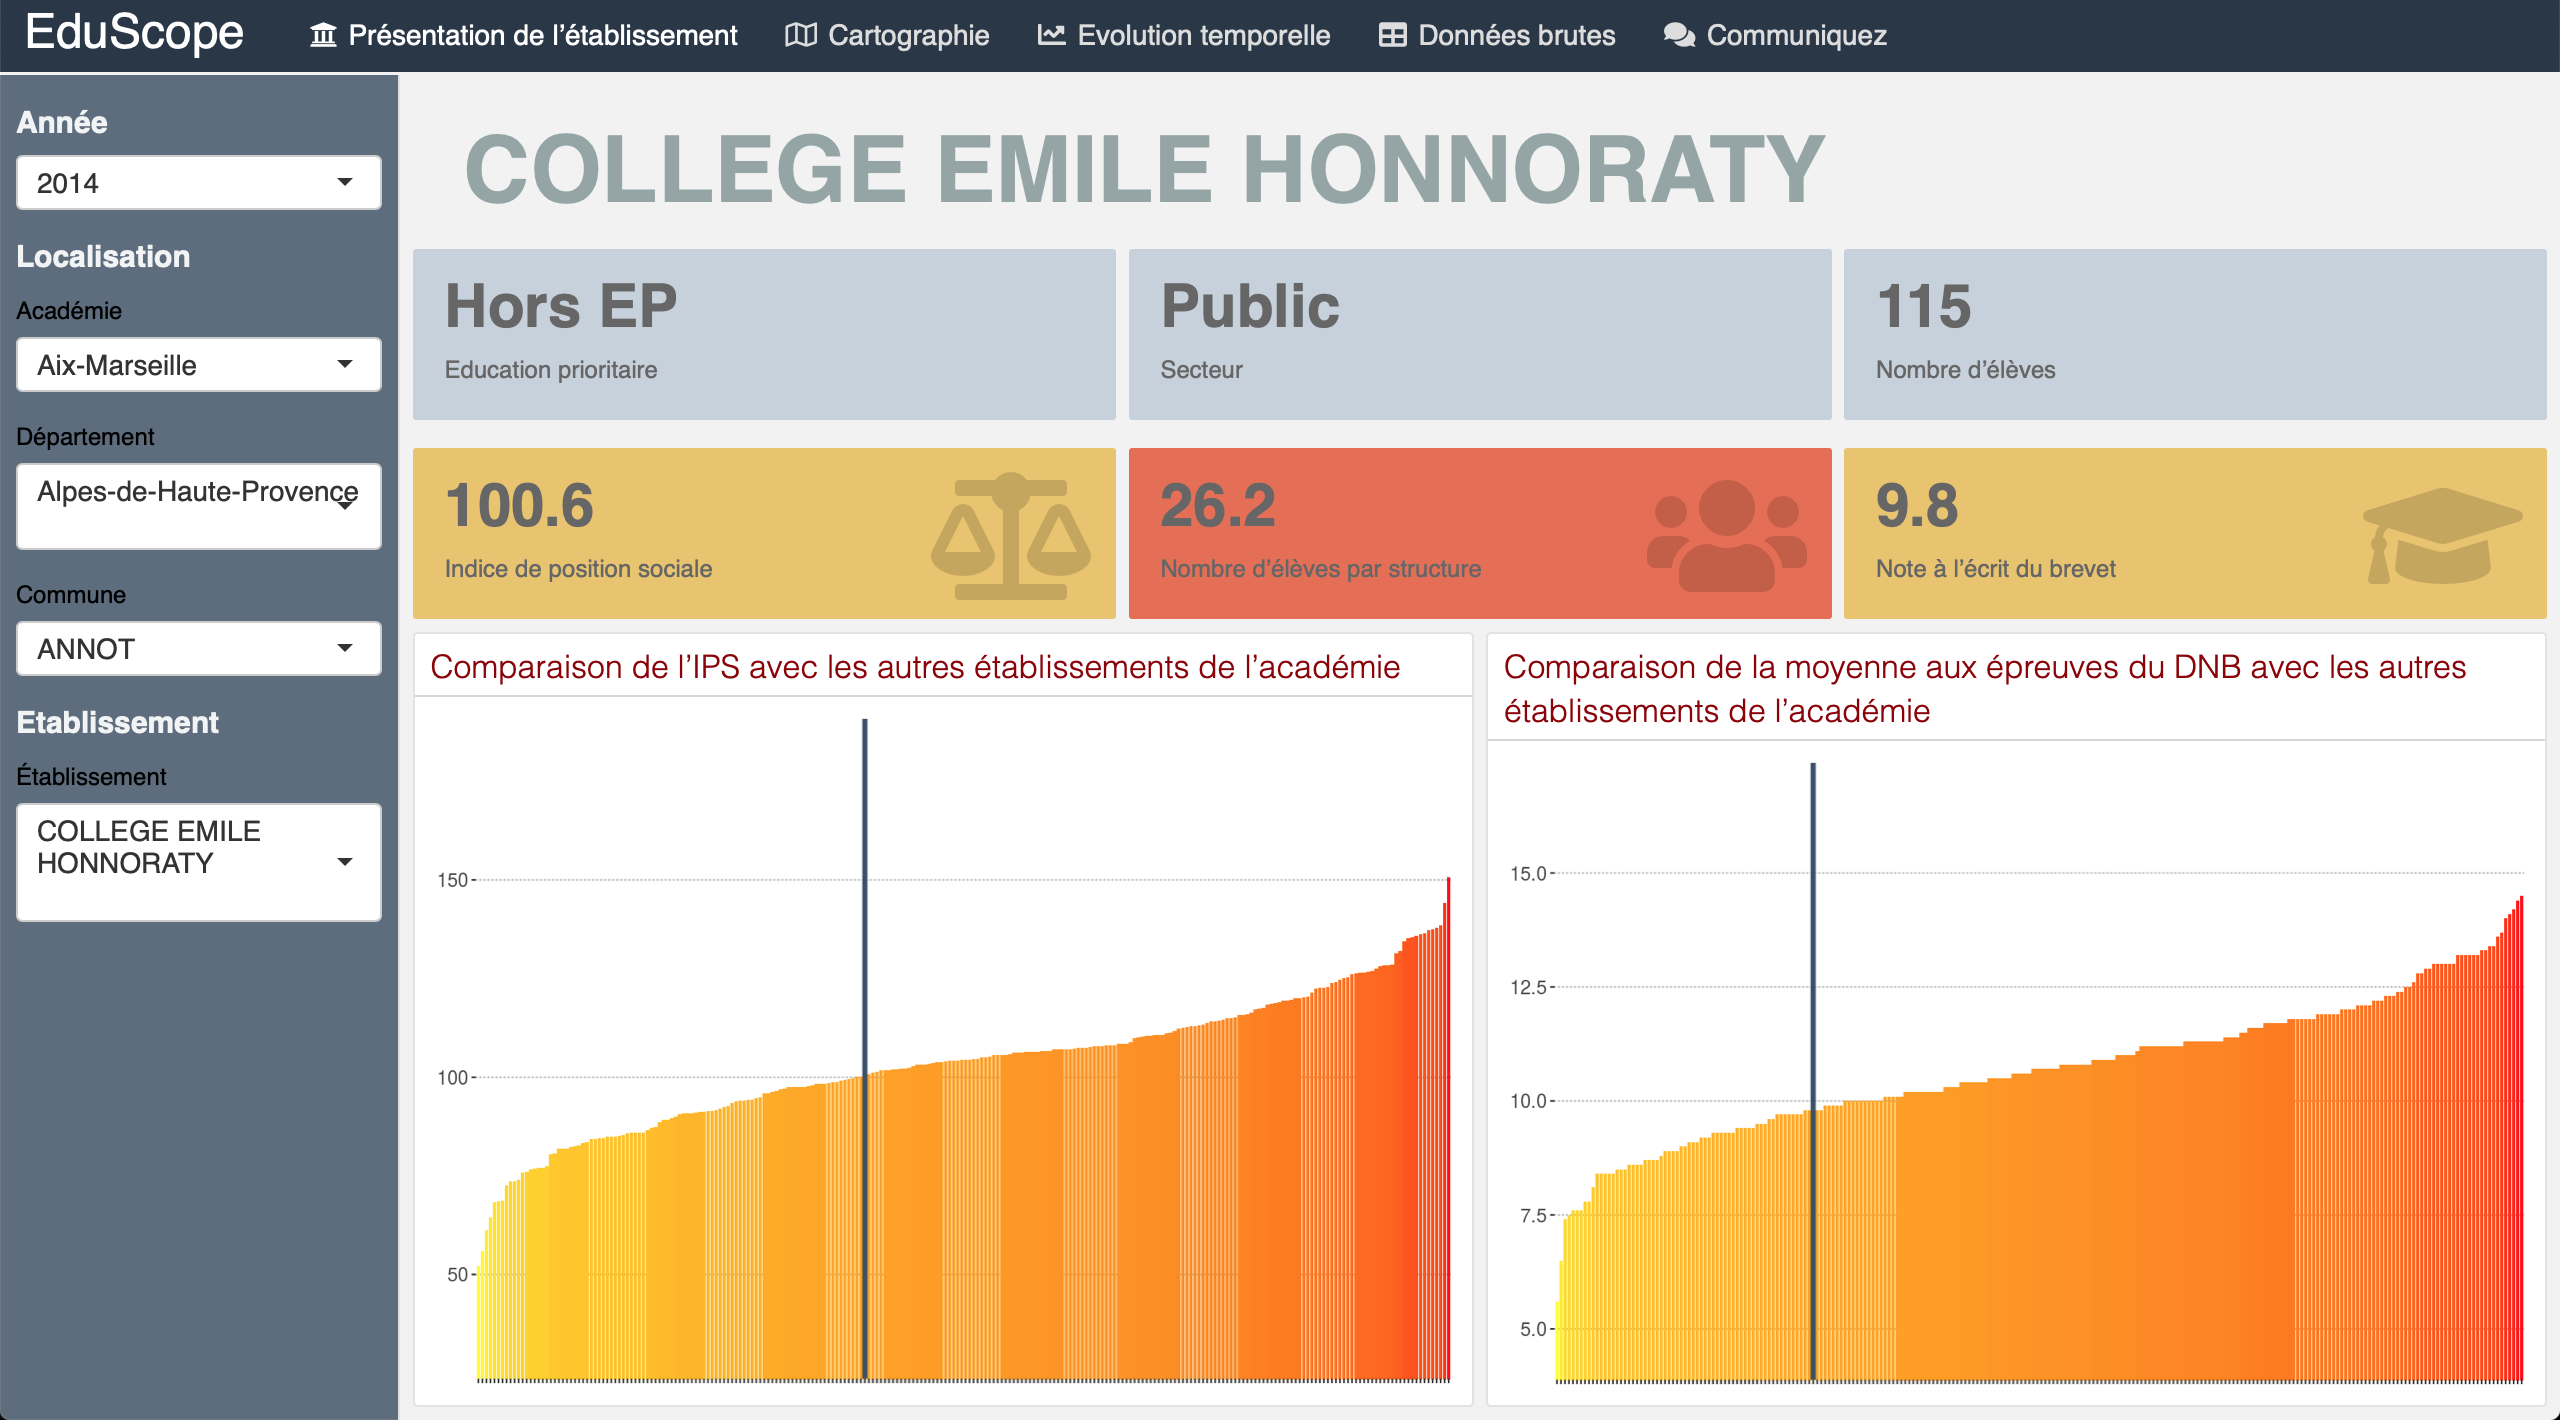
\includegraphics[width=0.6\linewidth]{./img/eduscope} 

}

\caption{Vue synthétique des données disponibles par établissement.}\label{fig:unnamed-chunk-8}
\end{figure}

La plateforme permet également de visualiser l'évolution des différents
indicateurs dans le temps, mais aussi de faire circuler des informations
qualitatives entre utilisateurs.

\subsection{Open}\label{open}

\begin{quote}
\href{http://datavizchallenge.fr/t/defi-n-2-open-placer-la-data-et-les-eleves-au-du-processus-de-decision/89/6}{Lien
vers la documentation}
\end{quote}

\textbf{Contexte} : L'identité d'un établissement se résume souvent à
bien plus que ses indicateurs de performance. Elle peut aussi être
enrichie par son dynamisme interne et son écosystème socio-culturel
(proximité des lieux culturels, des infrastructures sportives,
d'associations, etc). Ces informations peuvent être particulièrement
utiles pour les élèves, qui disposent actuellement de peu d'outils pour
comprendre et prendre part à la vie de leur établissement et tirer
profit de son environnement.

Comment remettre les élèves au centre de l'identité et du processus de
décision des établissements ?

\textbf{Produit final} : Maquette de plateforme participative accessible
aux élèves pourvus d'un identifiant. Elle leur donne la possibilité de
réagir, partager leur ressenti, mais aussi d'émettre des propositions
pour améliorer la vie dans leur établissement.

Elle propose également une vision géolocalisée de l'établissement
permettant aux élèves d'identifier les offres pédagogiques, sportives et
culturelles à proximité, puis d'effectuer un retour d'expérience sur ces
offres.

\begin{figure}

{\centering 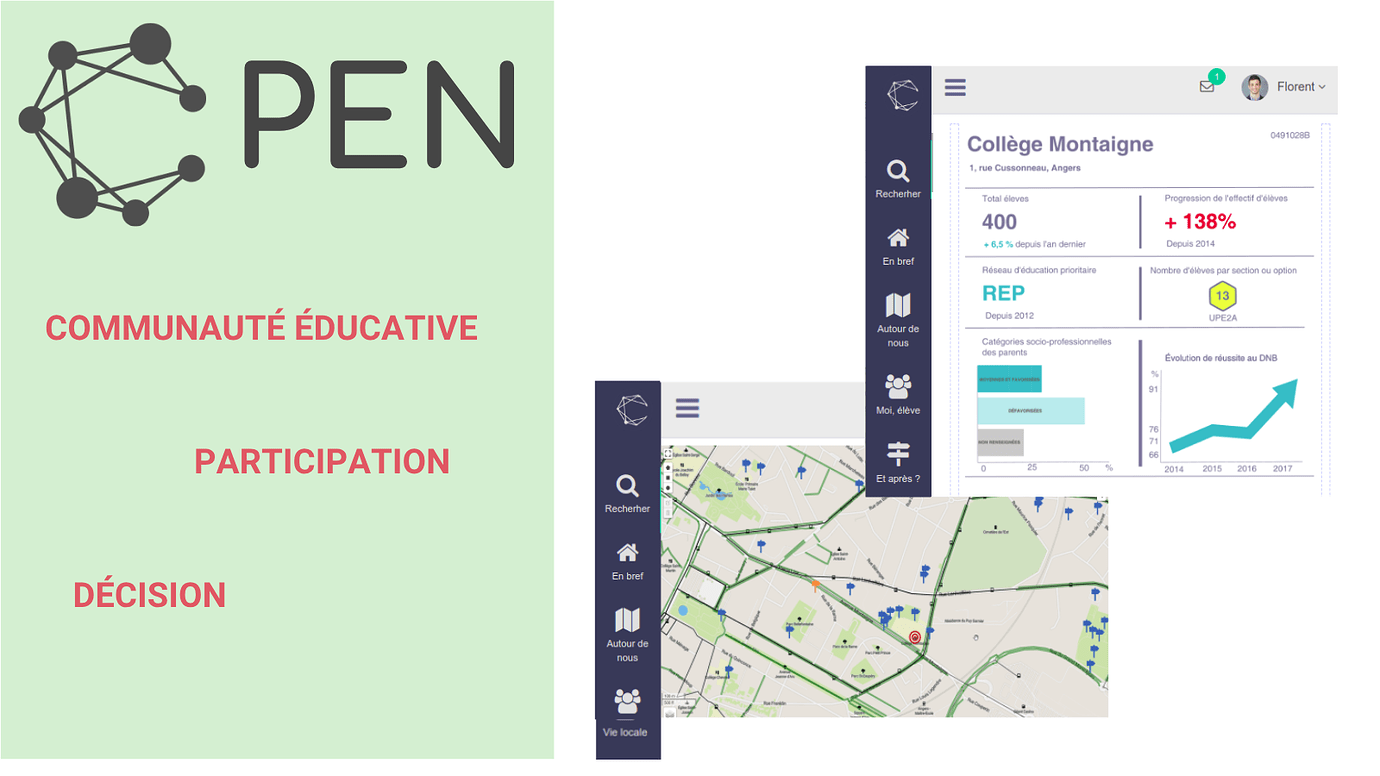
\includegraphics[width=0.7\linewidth]{./img/open} 

}

\caption{Visuels du service OPEN.}\label{fig:unnamed-chunk-9}
\end{figure}

\subsection{Antisèche}\label{antiseche}

\begin{quote}
\href{http://datavizchallenge.fr/t/dataviz-r-shinyapp/74}{Lien vers la
documentation}
\end{quote}

\textbf{Contexte : }Lors de leurs déplacements, les recteurs et agents
du ministère ont besoin d'accéder rapidement à une vue synthétique des
principales caractéristiques d'un établissement, où qu'ils soient et
sans avoir forcément accès à un poste informatique. Ils cherchent
également à pouvoir développer une vision comparative des informations
entre les établissements, afin de pouvoir orienter leur discours et
prise de décision.

Comment concevoir un outil répondant à l'ensemble de ces besoins ?

**Produit final¨: Prototype d'application permettant une visualisation
géolocalisée des établissements, et d'accéder à une présentation
synthétique et ergonomique de leurs indicateurs principaux (nombre
d'élèves, taux de réussite au Brevet des Collèges, cours et options
proposées, capacité d'accueil, nombre d'enseignants par élève, etc).

L'outil propose également une vision évolutive de ces indicateurs dans
le temps, ainsi qu'une fonction de filtrage permettant de cibler les
variables d'intérêt ¨

\begin{figure}

{\centering 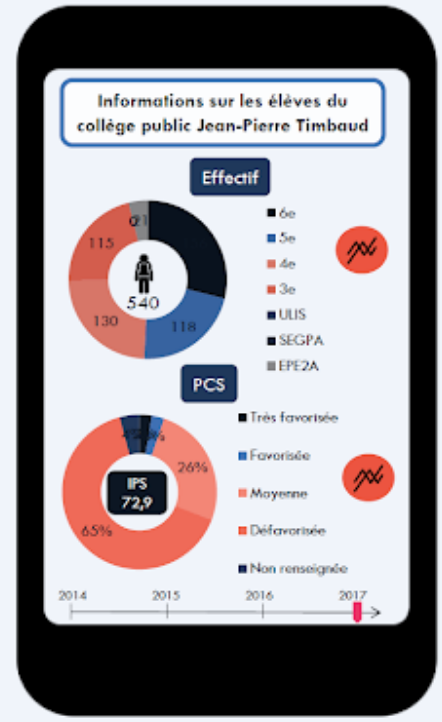
\includegraphics[width=0.4\linewidth]{./img/antiseche} 

}

\caption{Maquette du service Antisèche}\label{fig:unnamed-chunk-10}
\end{figure}

\section{DÉFI N°3 : «Carto du numérique dans les
territoires»}\label{defi-n3-carto-du-numerique-dans-les-territoires}

\subsection{Cadrage du défi}\label{cadrage-du-defi-2}

eCarto est un outil créé par la Caisse des Dépôts, en partenariat avec
le ministère de l'Education nationale et de la Jeunesse et les
associations de collectivités. Il permet de visualiser le déploiement du
numérique éducatif dans chacun des 63 000 établissements scolaires, en
rassemblant les données open data sur la connectivité, l'équipement, les
ressources et les expérimentations. Il a vocation à être un outil
permettant : * au plus grand nombre de s'informer sur l'état du
numérique éducatif en France ; * aux décideurs publics d'ajuster
l'accompagnement des académies et des collectivités en matière de
déploiement du numérique éducatif ; * aux acteurs des politiques
éducatives locales d'identifier plus facilement les établissements où un
enseignement à distance serait possible dans de bonnes conditions.

\textbf{Objectifs} : faciliter l'appropriation des données relatives au
déploiement du numérique éducatif en France en augmentant l'outil
eCarto.

\textbf{3 questions pour démarrer le DataViz Challenge :} * Quelles sont
les disparités territoriales observables ? * Quelles données
complémentaires et extensions possibles pour enrichir la représentation
du niveau de maturité numérique d'un territoire ? * Quelles mises en
perspective possibles entre niveau de maturité numérique et niveau
d'enclavement / isolement géographique d'un territoire ?

\subsection{🏆Alain Jette}\label{alain-jette}

\begin{quote}
\textbf{Projet retenu par le jury pour le défi 3}
\textbf{\href{https://drive.google.com/drive/folders/1dkZBb5xC6zCmAiD-EKUGl0TThzRDolEe}{Lien
vers la documentation}}
\end{quote}

\textbf{Contexte :}Les établissements scolaires regorgent de projets
pédagogiques. Cependant, ceux-ci ont souvent peu de visibilité au sein
de leur territoire, ce qui peut limiter leur portée et l'investissement
qu'ils reçoivent en ressources humaines, financières et matérielles
nécessaires à leur portage. Cette opacité peut également jouer sur
l'image d'un établissement, les indicateurs standards ne permettant pas
d'en valoriser la prise d'initiatives, la créativité et le dynamisme
internes.

Comment rendre visible les projets pédagogiques sur un territoire afin
de développer l'inspiration , le partenariat et l'action de tous ?

\textbf{Produit final}: Maquette de carte multidimensionnelle et
collaborative des projets pédagogiques. Son design inspiré de l'univers
de Lego invite à concevoir les projets pédagogiques comme des
co-constructions. L'outil recense l'ensemble des projets organisés sur
un territoire (ici l'Académie de Dijon) ainsi que leur description.

\begin{figure}

{\centering 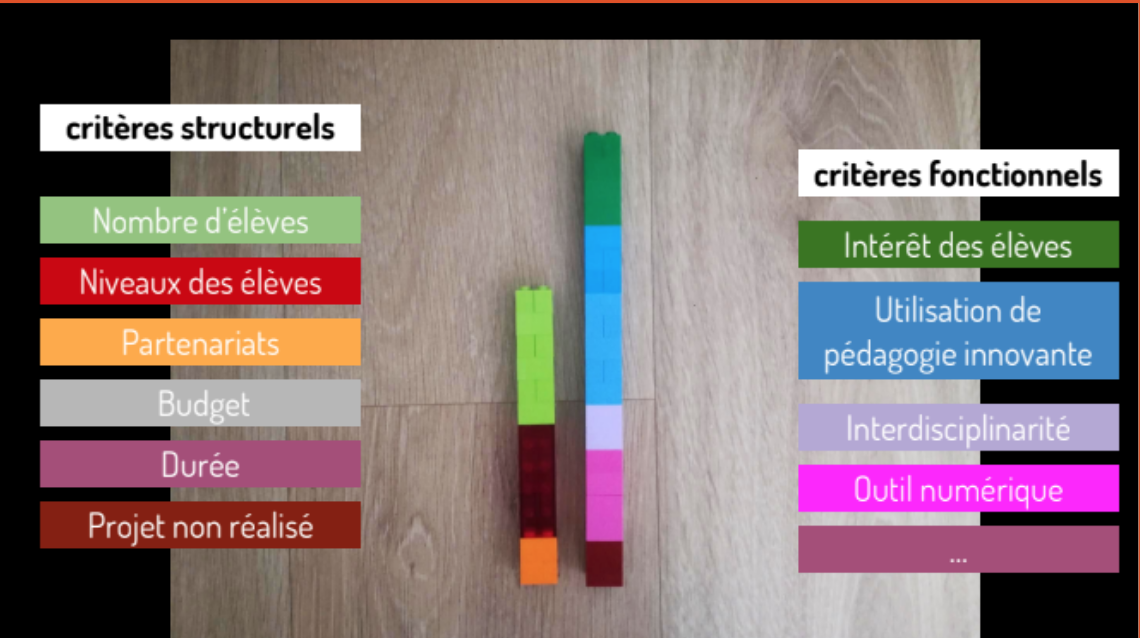
\includegraphics[width=0.7\linewidth]{./img/alainjette} 

}

\caption{Illustrations du projet à partir de LEGO.}\label{fig:unnamed-chunk-11}
\end{figure}

Il offre également un module de recherche ciblée selon des critères
structurels (nombre d'élèves, budget, durée, etc) et fonctionnels
(utilisation des outils numériques, pédagogie innovante,
interdisciplinarité, etc). Cette recherche affinée est amenée à
faciliter la conclusion de partenariats et le partage de ressources
entre les équipes pédagogiques, mais peut aussi aider le recteur à
piloter son académie. Cela permet finalement de valoriser aussi bien le
projet que son établissement d'accueil.

\subsection{Panser la fracture
numérique}\label{panser-la-fracture-numerique}

\begin{quote}
\href{https://drive.google.com/drive/folders/1dkZBb5xC6zCmAiD-EKUGl0TThzRDolEe}{Lien
vers la documentation}
\end{quote}

\textbf{Contexte} : Les établissements scolaires sont les premiers
touchés par les effets de la ``fracture numérique''. Ces inégalités ne
relèvent pas seulement de l'accès aux équipements informatiques, elles
sont également induites par d'autres paramètres tels que la couverture
numérique de l'établissement, sa catégorie (ex: REP/REP+), ses
financements, son nombre d'enseignants, leurs formations\ldots{}

Comment mesurer et visualiser les écarts de facilité d'accès au
numérique entre différents établissements en tenant compte de tous ces
paramètres pour mieux adapter les réponses politiques et évaluer leurs
impacts?

\textbf{Produit final} : Maquette de cartes en relief permettant de
visualiser un indicateur synthétique d'accès au numérique, d'en cibler
les composantes et de les comparer à ceux des établissements
environnants et à la moyenne nationale.

\begin{figure}

{\centering 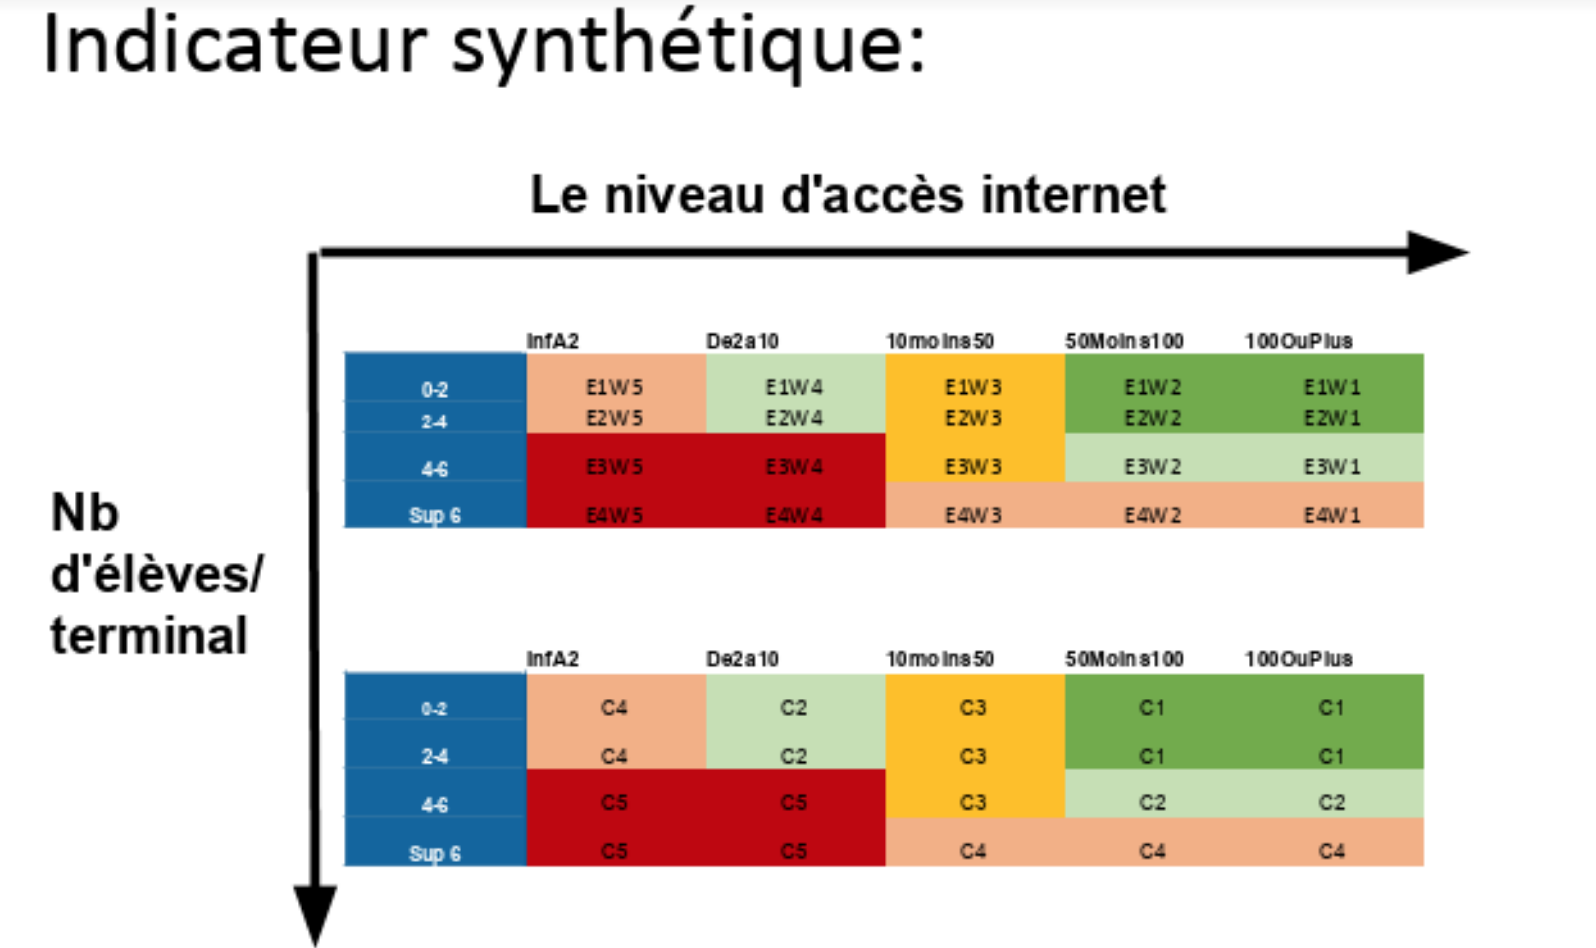
\includegraphics[width=0.7\linewidth]{./img/pan} 

}

\caption{Indicateur synthétique sur accès au numérique}\label{fig:unnamed-chunk-12}
\end{figure}

\textbf{Méthode} :

\begin{itemize}
\tightlist
\item
  Création d'un indicateur synthétique (Numeriscor) en croisant les
  données existantes (débit internet, nb d'élève/terminal, vétusté des
  équipements, etc) et d'autres données aujourd'hui difficilement
  trouvables (qualification des professeurs C2i2e, nombre de formations
  sur le numérique, etc)
\item
  intégration de l'indicateur à eCarto et à la fiche de chaque
  établissement.
\item
  création d'une moyenne départementale et nationale sur eCarto pour
  pouvoir facilement positionner un établissement par rapport aux autres
  et identifier ceux en difficultés
\end{itemize}

\chapter{Les principes d'un sprint data réussi}\label{principes}

\section{Historique : d'où viennent les data sprints
?}\label{historique-dou-viennent-les-data-sprints}

\section{Hackathon, data sprints, dataviz challenge, data camps :
définition des
formats}\label{hackathon-data-sprints-dataviz-challenge-data-camps-definition-des-formats}

\section{Les 3 ingrédients essentiels : défis, données,
participants}\label{les-3-ingredients-essentiels-defis-donnees-participants}

\section{Les facteurs clés de succès}\label{les-facteurs-cles-de-succes}

\chapter{La préparation du data sprint}\label{preparation}

\section{Les principaux points
d'attention}\label{les-principaux-points-dattention}

\section{Présentation du retroplanning
type}\label{presentation-du-retroplanning-type}

\section{La mobilisation des mentors}\label{la-mobilisation-des-mentors}

\section{Le recrutement des
participants}\label{le-recrutement-des-participants}

\section{La préparation des données}\label{la-preparation-des-donnees}

\section{La mise en place des espaces de discussion et de
documentation}\label{la-mise-en-place-des-espaces-de-discussion-et-de-documentation}

\chapter{L'animation du data sprint}\label{animation}

\section{Les trois temps créatifs : inspiration, idéation,
prototypage}\label{les-trois-temps-creatifs-inspiration-ideation-prototypage}

\section{Les ateliers de formation}\label{les-ateliers-de-formation}

\section{Les temps de pause et
d'inspiration}\label{les-temps-de-pause-et-dinspiration}

\section{La documentation des
projets}\label{la-documentation-des-projets}

\section{Quelques questions
logistiques}\label{quelques-questions-logistiques}

\chapter{La restitution et la suite}\label{la-restitution-et-la-suite}

\section{Les présentations des
projets}\label{les-presentations-des-projets}

\section{La délibération du jury}\label{la-deliberation-du-jury}

\section{L'accompagnement à donner}\label{laccompagnement-a-donner}

\bibliography{book.bib,packages.bib}


\end{document}
